\chapter{Methodology}
\section{Threat Modeling}
Threat modeling is a technique that allows us to detect and address top threats that can have a significant impact on the application \citep{threat_modeling}. Similarly, this web application uses the STRIDE threat model to discover threats. The threats in the table will be tested against the system to detect any vulnerabilities.
Using the DFD (see figure \ref{fig:dfd}), we can list some threats utilizing the model.

\begingroup
\centering
\setlength{\tabcolsep}{6.5pt} % Default value: 6pt
\renewcommand{\arraystretch}{1.8} % Default value: 1
\begin{longtable}{ |p{7cm}| p{8cm} |}
\caption{STRIDE Modeling}
    \label{table:spoofing}
\hline
\rowcolor{grey!15}
\textbf{STRIDE} & \textbf{Threats}\\
\hline
Spoofing & \begin{enumerate}
    \item DNS spoofing allowing to redirect to a malicious site.
    \item Ip Spoofing \citep[p.~2]{ip_spoofing}
\end{enumerate} \\
\hline
Tampering & \begin{enumerate}
    \item Upload malicious files.
    \item Cross-Site Request Forgery. \citep[p.~538]{crsf}
\end{enumerate} \\
\hline
Repudiation & \begin{enumerate}
    \item Malicious activities are not tracked.
\end{enumerate} \\
\hline
Information Disclosure & \begin{enumerate}
    \item SQL Injection into the database.
    \item Various network information is public.
\end{enumerate} \\
\hline
Denial of Service & \begin{enumerate}
    \item The CMS site is hit with a DoS attack.
\end{enumerate} \\
\hline
Elevation of Privileges & \begin{enumerate}
    \item Unauthorized users with admin privileges are added.
\end{enumerate} \\
\hline
\end{longtable}
\endgroup

\begin{figure}[h!]
\centering
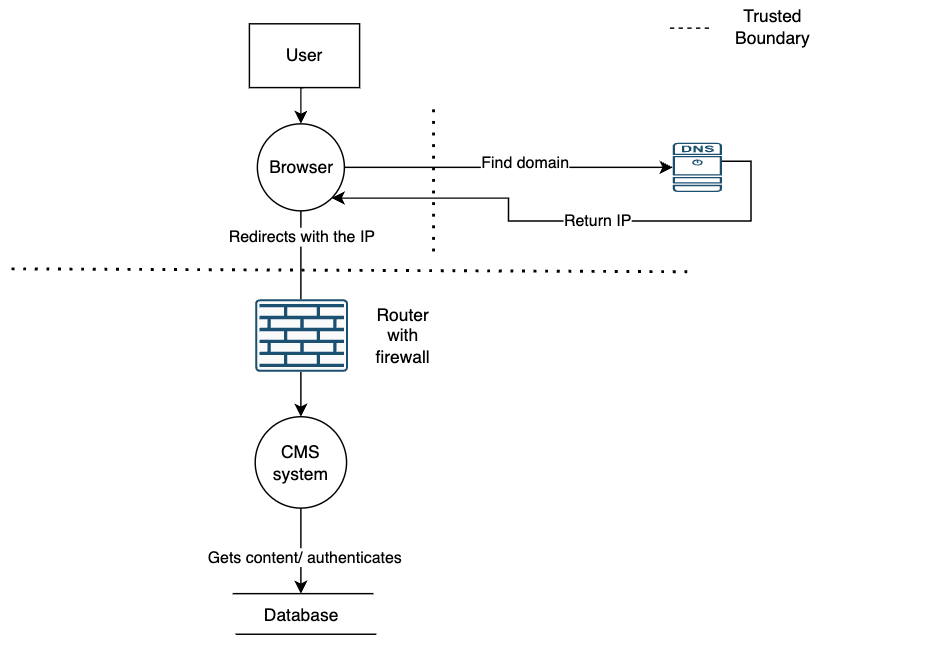
\includegraphics[width=\textwidth, height=280px]{pics/dfd.png}
\caption{DFD level 0 for the CMS system}\label{fig:dfd}
\end{figure}


\section{Vulnerability Assessment}
For the vulnerability assessment, the automated tools (see table \ref{table:tools}) mentioned in the baseline analysis were used to scan for known threats and misconfigurations of the CMS system using the adversary behaviors defined in MITRE Enterprise ATT\&CK matrix \citep[p.~158]{xiong2022cyber}.

\begin{comment}
Additionally, the assessment and reconnaissance are performed using the MITRE Enterprise ATT\&CK matrix \citep{mitre_url}, as this model describes the adversary behaviors that measure the system's resilience at an enterprise level \citep[p.~158]{xiong2022cyber}.
\end{comment}



\begingroup
\centering
\setlength{\tabcolsep}{6.5pt} % Default value: 6pt
\renewcommand{\arraystretch}{1.8} % Default value: 1
\begin{longtable}{ |p{5cm}| p{10cm} |}
\caption{Results from the tools used in the assessment}
    \label{table:tools}
\hline
\rowcolor{grey!15}
\textbf{Tool}  & \textbf{Result}\\
\hline
Cmsmap &  \begin{enumerate}
    \item CMS Detected version detected.
    \item PHP version detected.
\end{enumerate}\\
\hline
Metasploit \& Nmap &  \begin{enumerate}
    \item Discovered network misconfigurations.
    \item Tested against major CRM threats (i.e., SQL injection, XSS, RCE, Directory traversal) mentioned in the baseline analysis.
\end{enumerate}\\
\hline
DNSrecon &  \begin{enumerate}
    \item Performed reverse lookup and CDN detection.
    \item Performed DNS Zone transfer.
    \item Performed Cache Snooping and DNS Recursion.
    \item Performed Zone walking.
\end{enumerate}\\
\hline
\end{longtable}
\endgroup

\section{GDPR Analysis}
Using the GDPR compliance checklist, the website is evaluated for compliance with GDPR \citep{gdpr_checklist}. Failure to comply with GDPR rules with severe violations can be fined up to 4\% of the total turnover, or €20 million \citep[p.~32]{eu_fines}. Table \ref{table:gdpr} summarizes the discovered GDPR compliance results for the CMS system.

\newpage
\begingroup
\centering
\setlength{\tabcolsep}{6.5pt} % Default value: 6pt
\renewcommand{\arraystretch}{1.8} % Default value: 1
\begin{longtable}{ |p{3cm}|p{5cm}| p{7cm} |}
\caption{GDPR Assessment}
    \label{table:gdpr}
\hline
\rowcolor{grey!15}
\textbf{Article GDPR} & \textbf{Name}  & \textbf{Status}\\
\hline
Art.3 & Representative of Controller in the European Union  &  \begin{enumerate}
    \item A representative in the European Union is required as the CRM is hosted in the United States and processes personal data. The presence of the officer is unknown.
\end{enumerate}\\
\hline
Art.12 & Transparent privacy policy use, with the subject's consent.  &  \begin{enumerate}
    \item A consent layer for informing users of the information the cookies collect is missing.
    \item Granular consent is also not present.
    \item Privacy policy of the website link is not present.
\end{enumerate}\\
\hline
Art.25 & Data Protection by Design and default.  &  \begin{enumerate}
    \item The databases containing personal data are available on the public internet, creating a risk of personal data breaches.
    \item The accounts are protected with an authentication mechanism.
\end{enumerate}\\
\hline
Art.32 & Security of Processing.  &  
\begin{enumerate}
    \item Unencrypted email servers with ports (110, 143, 465, 587, and 2525) are used and are susceptible to man-in-the- middle-attacks.
    \item The CRM https website uses SSL-encrypted connections. 
\end{enumerate}\\
\hline
Art.33 \& 34 & Notification of breaches.  &  
\begin{enumerate}
    \item Logging and monitoring to detect unusual behaviors are required but cannot be confirmed.
    \item Incident response within 72 hours of a breach is required but cannot be confirmed.
\end{enumerate}\\
\hline
Art.38 & Presence of Data Protection Officer.  &  
\begin{enumerate}
    \item A data protection officer handling critical breach incidents is required. The availability of the DPO is unknown.
\end{enumerate}\\
\hline
\end{longtable}
\endgroup

